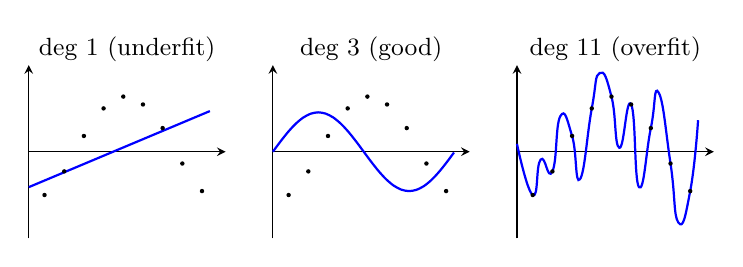
\begin{tikzpicture}[scale=0.5,>=stealth]
% three panels: deg1 underfit / deg3 good / deg11 overfit
\begin{scope}
\draw[->] (0,0)--(5,0); \draw[->] (0,-2.2)--(0,2.2);
\node at (2.5,2.6) {\small deg 1 (underfit)};
\draw[blue,thick,domain=0:4.6] plot (\x,{-0.9+0.42*\x});
\foreach \p in {(0.4,-1.1),(0.9,-0.5),(1.4,0.4),(1.9,1.1),(2.4,1.4),(2.9,1.2),(3.4,0.6),(3.9,-0.3),(4.4,-1.0)} \fill \p circle (1.6pt);
\end{scope}
\begin{scope}[xshift=6.2cm]
\draw[->] (0,0)--(5,0); \draw[->] (0,-2.2)--(0,2.2);
\node at (2.5,2.6) {\small deg 3 (good)};
\draw[blue,thick,domain=0:4.6,smooth] plot (\x,{sin(\x*78)});
\foreach \p in {(0.4,-1.1),(0.9,-0.5),(1.4,0.4),(1.9,1.1),(2.4,1.4),(2.9,1.2),(3.4,0.6),(3.9,-0.3),(4.4,-1.0)} \fill \p circle (1.6pt);
\end{scope}
\begin{scope}[xshift=12.4cm]
\draw[->] (0,0)--(5,0); \draw[->] (0,-2.2)--(0,2.2);
\node at (2.5,2.6) {\small deg 11 (overfit)};
\draw[blue,thick,domain=0:4.6,smooth,tension=0.9]
 plot coordinates {(0,0.2)(0.4,-1.1)(0.6,-0.2)(0.9,-0.5)(1.1,0.9)(1.4,0.4)(1.6,-0.7)(1.9,1.1)(2.1,2.0)(2.4,1.4)(2.6,0.1)(2.9,1.2)(3.1,-0.9)(3.4,0.6)(3.6,1.5)(3.9,-0.3)(4.1,-1.8)(4.4,-1.0)(4.6,0.8)};
\foreach \p in {(0.4,-1.1),(0.9,-0.5),(1.4,0.4),(1.9,1.1),(2.4,1.4),(2.9,1.2),(3.4,0.6),(3.9,-0.3),(4.4,-1.0)} \fill \p circle (1.6pt);
\end{scope}
\end{tikzpicture}
